% !TEX root = ../main.tex

This section will describe the implementation of the backend as well as the frontend. Implementation diagrams, code examples, and technical descriptions will be used. 

\subsection{Java Spring REST Backend}
To support the system functionality a Java RESTful service was developed using Spring. The reasoning behind using a REST backend is that the service can be consumed by any client that supports HTTP. Thus allowing for a web client as well as an android application to communicate with the backend. The endpoints for the service was implemented in accordance to the implementation class diagram \ref{fig:backend_class_diagram}. 

\begin{figure}[hbt]
\centering
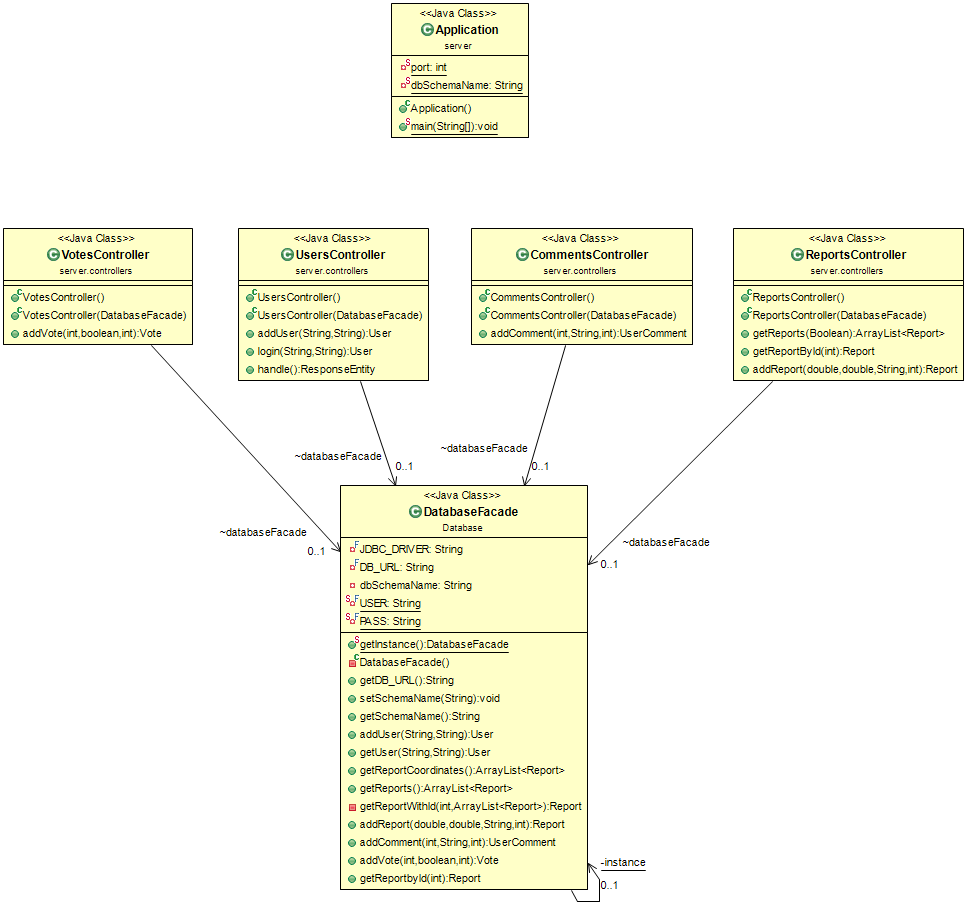
\includegraphics[width=\linewidth]{images/Class_backend_diagram}
\caption{Server side class diagram.}\label{fig:backend_class_diagram}
\end{figure}

%\todo[inline]{explain the diagram in \autoref{fig:backend_class_diagram}}
\autoref{fig:backend_class_diagram} shows the classes implemented in the backend. All the controller have two constructors; an empty constructor and a constructor that takes a DatabaseFacade class as a parameter. This is used to enable unit testing of the REST controllers by allowing dependency injection to mock the database facade. The database facade contains the logic for communicating with a MySQL database using JDBC thus achieving persistence for the application. 

\begin{description}
\item [The VotesController] lets users add an up- or downvote to reports.
\item [The UsersController] lets unregistered users sign up and lets registered users login.
\item [The CommentsController] lets users add comments to reports.
\item [The ReportsController] lets users get all reports, get a report by id, and add a new report.
\end{description}

\begin{listing}[H]
\caption{The ReportsController in Java Spring REST}\label{lst:restController}
%\todo[inline]{change the caption of Code Snippet \ref{lst:restController}}
\begin{minted}{java}
@RestController
@RequestMapping(value = "/api")
public class ReportsController {

    @RequestMapping(value = "/reports", params = {"only-coordinates"})
    public ArrayList<Report> getReports(@RequestParam(value="only-coordinates")
    Boolean onlyCoordinates) {
        if (onlyCoordinates) {
            return databaseFacade.getReportCoordinates();
        } else {
            return databaseFacade.getReports();
        }
    }
}
\end{minted}
\end{listing}

In Spring a REST endpoint is defined by using annotations. Specifically the annotation "\textit{@RestController}" is used to define an endpoint known as a  controller. This controller does not default to any URI, but another annotation is used for specifying the endpoint URI. The "\textit{@RequestMapping}" annotation is used for specifying URI's - the specific methods as well as the controller itself can use this annotation. All of the controllers maintain a reference to a database facade which is responsible for making the transactions with MySQL database to maintain persistent data.

\subsection{Databse}
The REST service is responsible for enabling HTTP access to the backend while the database facade is responsible for communicating with the MySQL database through JDBC. The database schema required to support the application is shown in figure \ref{fig:database_diagram}.

\begin{figure}[hbt]
\centering
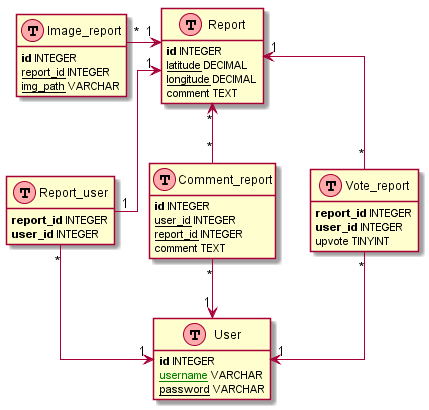
\includegraphics[width=.6\textwidth]{images/relational_model}
\caption{Relational Model that shows the database structure}\label{fig:database_diagram}
\end{figure}

The database diagram in figure \ref{fig:database_diagram} shows how the issue reports are connected to users and how the details of a report is interconnected. 

The \textbf{Image\_report} table contains a primary key \textit{id}, highlighted by underlining the column name, a foreign key \textit{id\_report}, highlighted by \textit{italic text}, and an \textit{img\_path} column. The \textit{img\_path} column is a string containing the relative path to an image file stored on the system. 

The \textbf{Comment\_report} table contains comments on reports submitted after the publishing of a report. The table contains two foreign keys that references the \textit{Report} and \textit{User} tables as well as a comment column.

The \textbf{Vote\_report} table contains the votes that users have cast on reports. The vote is saved as a TINYINT which is converted to a boolean value in Java. The table also contains two foreign keys - which is both primary keys as it is a weak entity - that references the \textit{Report} and \textit{User} tables.

The \textbf{Report\_user} table is a weak entity which bind reports to users by using two primary keys which are also foreign keys to the the \textit{Report} and \textit{User} tables.

The \textit{User} table contains the username and password of a user.

The \textit{Report} table contains the reports submitted by the users. The report table itself will contain the \textit{longitude} and \textit{latitude} of a problem as well as a problem description \textit{comment}.

\subsection{Android Client}
This section depicts how we implemented the android client. It describes which mobile sensing features we implemented and how we applied them into service. Secondly, it lists employed energy efficiency and resource adaptability tactics. Finally, we show user interface and describe some of the application flow with the help of screenshots of the android activities.

\subsubsection{Sensing}
We utilize two kinds of mobile sensing, activity and location. We use them to share data and inform people.

\textbf{Activity Sensing} with ActivityRecognitionClient  - extends GoogleApi
Once the user is logged in, the application will start with activity detection inside the TipNotificationService. Six types of user activities – \textit{UNKNOWN}, \textit{IN\_VEHICLE}, \textit{ON\_BICYCLE}, \textit{ON\_FOOT}, \textit{STILL} and \textit{TILTING} - are assessed continuously in the background.

ActivityRecognitionContainer is responsible for categorizing the \textit{ON\_FOOT} activity by fusing activities \textit{ON\_FOOT}, \textit{RUNNING} and \textit{WALKING}. It also serves as an interface for detected activities, storing type and confidence.

Sensor data processing is done inside TipDistanceHandler class.  If the activity is recognized as \textit{ON\_FOOT}, the class will determine if it should check for new report updates from the server. The default update interval for checking for new updates is 2 hours. If those 2 hours passed and the person is walking somewhere, the application will automatically download new reports. If the two hours have not passed, and the activity is still \textit{ON\_FOOT} , the class will calculate user distance to the reports. If the distance is less than 150 meters, the location service will increase its quality of delivery, precision. Simultaneously, it will compare the distance to the notification radius and if it’s less, notification will be triggered.

If the detected activity is any other than \textit{ON\_FOOT}, the TipDistanceHandler will attempt to decrease the location precision, to preserve power.
~\\

\textbf{Location sensing} with FusedLocationProviderClient - extends GoogleApi
TipLocationService is a background service which is started with user login and is stopped when the user logs out. First, googleApiClient is build and location request parameters (interval and priority) are set. The application then checks to see if it has the permissions to access location. If it does have that, the service starts the location updates through callbacks within the class and broadcasts it outside the class.

Location is forwarded to ReportsMapFragment (where Google map is displayed) and to TipNotificationService (to calculate distance between user and reports).


\subsubsection{Tactics}

The implemented tactics from design section are the following:
\begin{itemize}
\item Energy efficiency in sensing: Dynamic Duty Cycle, Sensor Replacement
\item Energy efficiency in processing: Event-based
\item Energy efficiency in sharing: Communication Selection
\item Resource adaptability in resource availability: Resource Selection
\end{itemize}

To show an example, \autoref{fig:sdLocChange} displays a sequence diagram of an Event-based tactic scenario, where the application changes the location service accuracy based on the users geographic proximity to nearby reports. 
% after user sends a trigger by walking somewhere and when he is in report radius, the change of precision happens.

\begin{figure}[H]
\centering
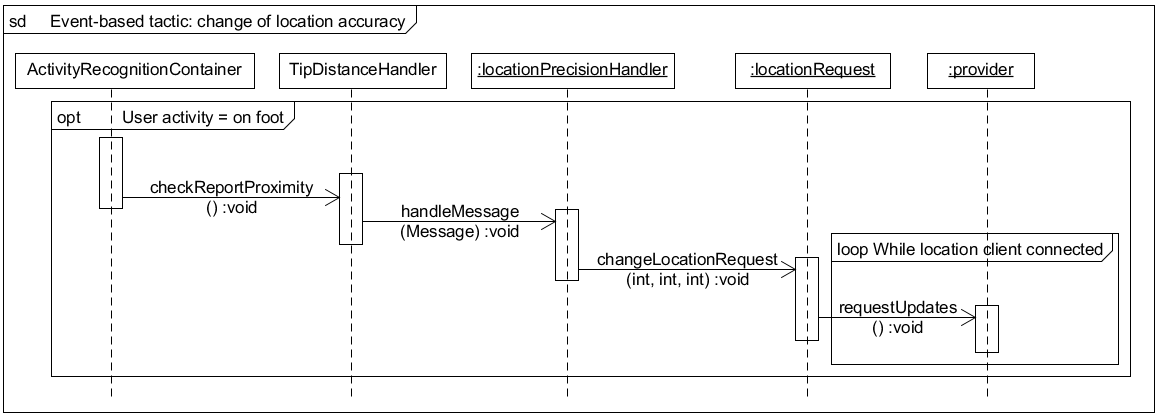
\includegraphics[width=\linewidth]{images/sdDiagram2}
\caption{Sequence diagram of the Location change Tactic} \label{fig:sdLocChange}
\end{figure}


\subsubsection{User Interface}
In the implemented User Interface, have built upon the User Interface from \autoref{sec:uidesign}. It now have functionality, handling of notifications of nearby reports, and commenting on reports. The implemented leaderboard is for demonstrative purposes only, and does not have any functionality.

\paragraph{The App Flow}~\\
After the non-registered user registers an account, he has the option to log into his account (1). 
When he logs in, he will be shown the map view (4) with his current location marked by a black triangle, and markers of existing reports will be displayed. 

The user can either use intuitive navigation by clicking on things, or sidebar navigation (2). 

To create a report, the user has to be in the location he wants to report it at (3). The location will be shown in the map view fragment inside activity, where description is also put before submission. 

Once the user walks by an existing report, the phone will vibrate and play a sound, and a notification will be shown (4). There, the user can confirm or deny the report, therefore helping us to validate it, or comment further on it.

\begin{figure}[H]
\centering
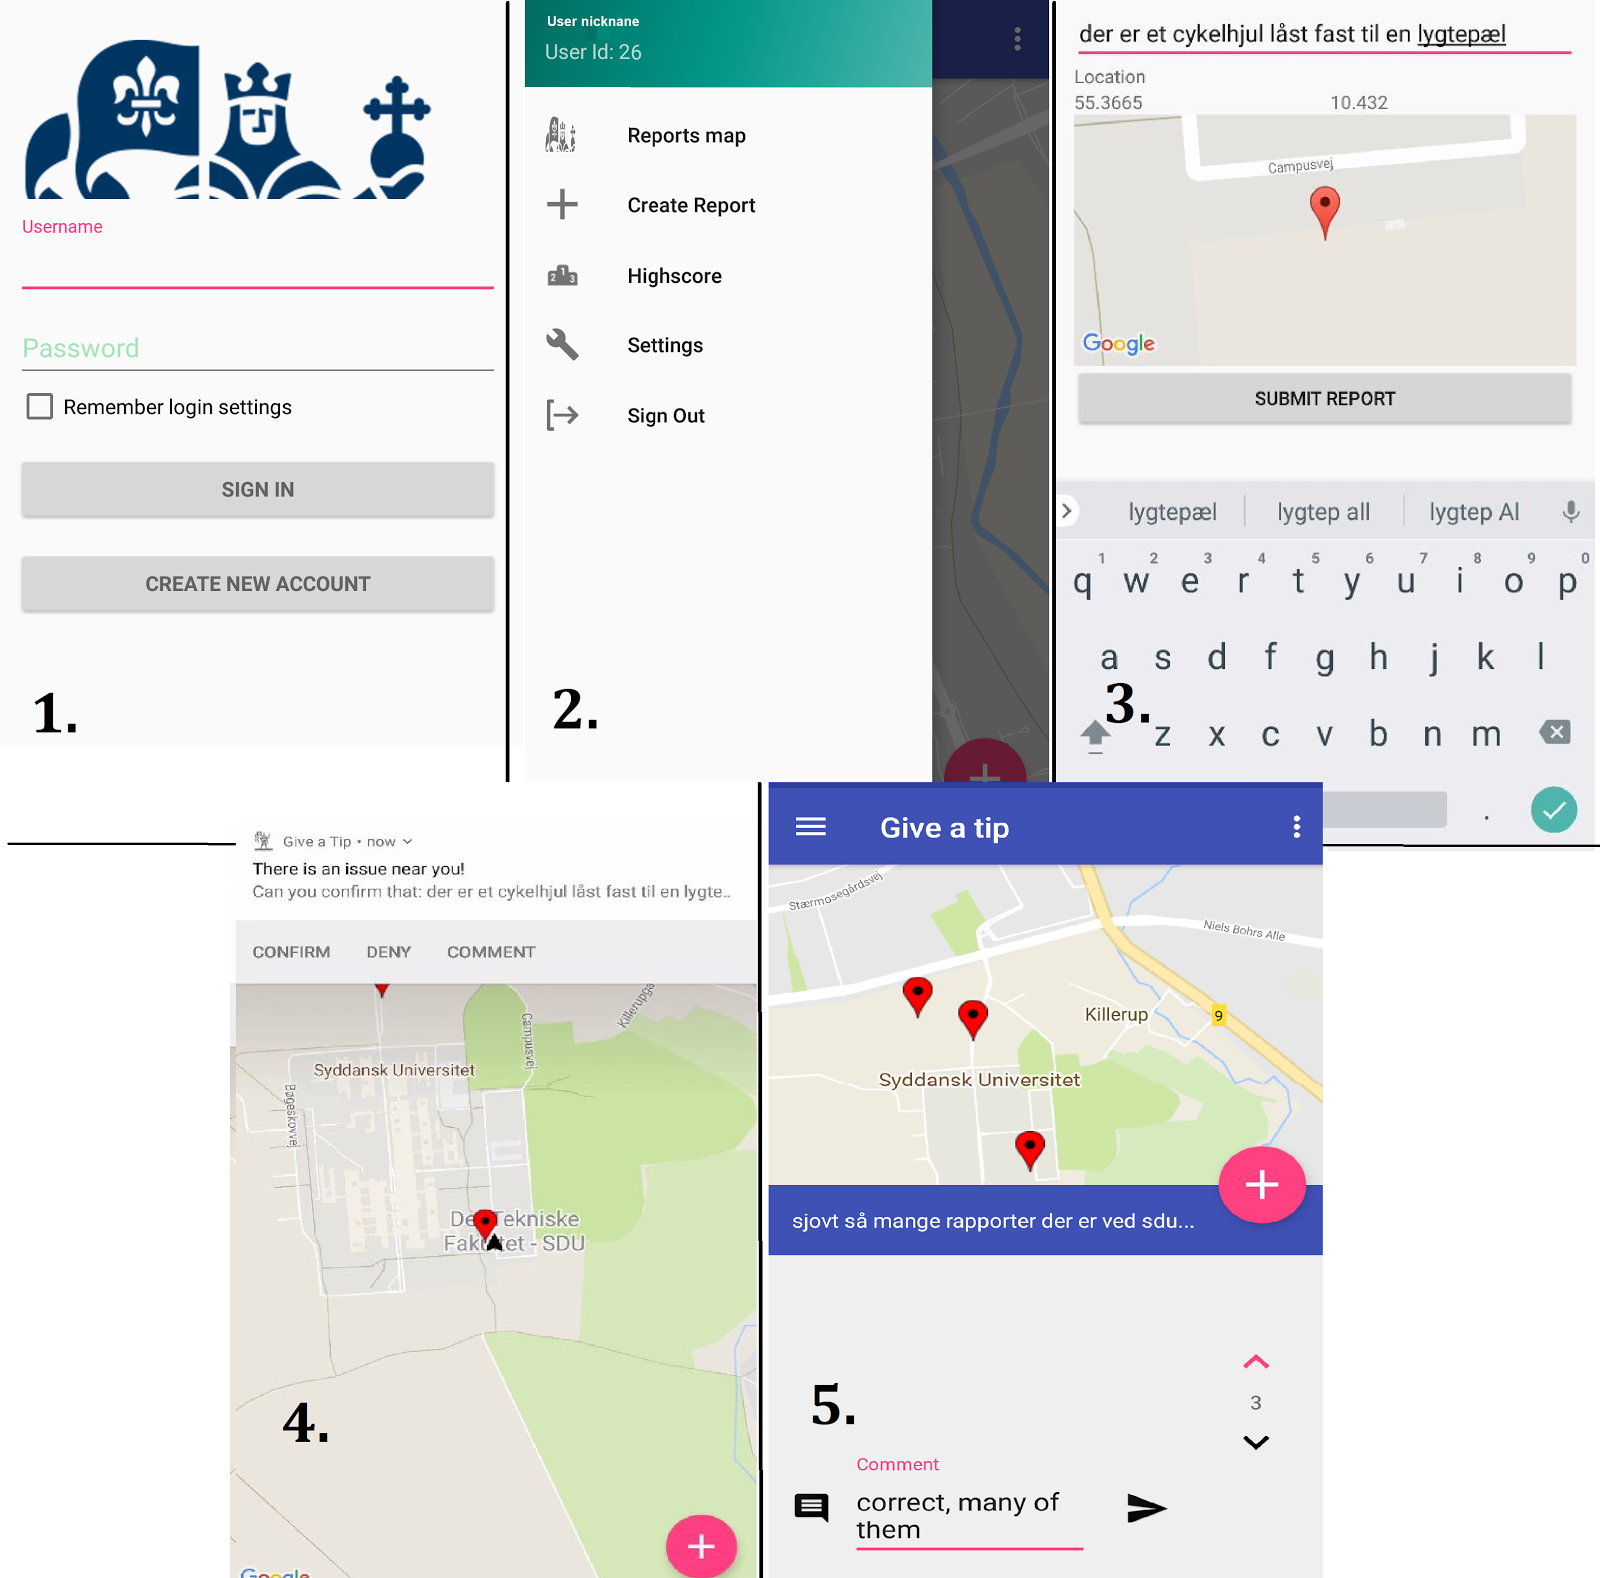
\includegraphics[width=\linewidth]{images/app_design.png}
\caption{Screenshots from the final prototype} \label{fig:appdesign}
\end{figure}


\vspace{3em}
\hrule
This section described the technical implementation of the system. A RESTful web service communicating with a MySQL database was developed to support HTTP clients - including the Android frontend. Android client was developed with activity and location sensing features, and with some of the architectural tactics described in design section. 

